\documentclass{beamer}
\usepackage{pgfpages}

\usepackage{amsmath}
\usepackage{amsthm}
\usepackage{amssymb, amstext, amsfonts, amscd, dsfont}

\usepackage{tikz}
\usepackage{tkz-euclide}

\usepackage{rotating}

\newcommand{\RR}{\mathbb{R}}
\newcommand{\QQ}{\mathbb{Q}}
\newcommand{\NN}{\mathbb{N}}

% -- differentials --
\renewcommand{\d}{\partial\mspace{2mu}} % partial diff
%\renewcommand{\d}{\mathrm{d}\mspace{2mu}}
\newcommand{\td}{\,\mathrm{d}}  % total diff
\newcommand{\tdfrac}[2]{\frac{\td #1}{\td #2}}
\newcommand{\pdfrac}[2]{\frac{\d #1}{\d #2}}


\usetheme{Copenhagen}
\useoutertheme{split}

\setbeameroption{show notes}
%\setbeameroption{show notes on second screen=right}

\graphicspath{{images/}}

\title{Measure Theory and Probability}

\begin{document}

\maketitle

\begin{frame}
  \tableofcontents{}
\end{frame}
\section{Background}

\begin{frame}{Why Measure Theory}
  \begin{itemize}
  \item Ca. 1900: What is the volume of a subset of $\RR^n$?
  \end{itemize}
  \note[item]{Around 1900, mathematicians tied to come up with a
    universal definition of the notion of volume.}
  \note[item]{For quite a long time, they were able to work with their
    intuitive feeling for volume. But the development of set theory
    forced them to be more precise about their understanding of volume.}
  \note[item]{To show you that this is not as trivial as one might think,
    I want to show you some examples}
\end{frame}
\begin{frame}{What is volume?}
  \begin{minipage}{0.45\linewidth}
    \begin{center}
      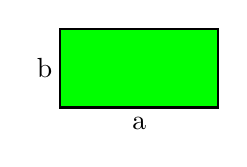
\begin{tikzpicture}[style=thick, fill=green]
        \draw[fill=green] (0,0) rectangle (2,1);
        \draw             (1.0, -0.2) node{a};
        \draw             (-0.2, 0.5) node{b};
      \end{tikzpicture}
    \end{center}
  \end{minipage}%
  \begin{minipage}{0.45\linewidth}
    $A = a \cdot b$
  \end{minipage}
  \note[item]{This one is quite clear. The volume of a rectangle with sides
   $a$ and $b$ should be $a\cdot b$. More exactly: If we take the volume of
   the unit square to be one and want the volume to be multilinear, than we
   get this.}
  \pause
  \begin{minipage}{0.45\linewidth}
    \begin{center}
      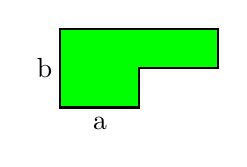
\begin{tikzpicture}[style=thick]
        \path[draw,fill=green] (0,0) -- (1,0) -- (1,0.5) -- (2, 0.5)
           -- (2,1) -- (0,1) -- cycle;
        \draw             (0.5, -0.2) node{a};
        \draw             (-0.2, 0.5) node{b};
      \end{tikzpicture}
    \end{center}
  \end{minipage}%
  \begin{minipage}{0.45\linewidth}
    $A = a \cdot b + \tfrac12 a \cdot b = \tfrac 32 \cdot a \cdot b$
  \end{minipage}
  \note[item]{This example is not that more complicated. Intuitively we
    expect the volume to be additive. Thus we can divide this object into
    two rectangles}
  \pause

  \begin{minipage}{0.45\linewidth}
    \begin{center}
      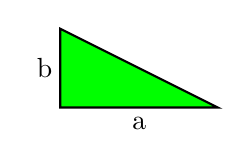
\begin{tikzpicture}[style=thick]
        \path[draw,fill=green] (0,0) -- (2,0) -- (0,1) -- cycle;
        \draw             (1.0, -0.2) node{a};
        \draw             (-0.2, 0.5) node{b};
      \end{tikzpicture}
    \end{center}
  \end{minipage}%
  \begin{minipage}{0.45\linewidth}
    $A = \tfrac12 a \cdot b$
  \end{minipage}
  \note[item]{This equation becomes clear, if we divide a rectangle into two
    triangles which we then intuitively assume to have the same volume.}
\end{frame}

\begin{frame}{What is volume?}
  \note[item]{Now what can we learn from the circle? Of course we all know that
    it's volume is $\pi r^2$, but how do we get this result? Obviously we cannot
    divide the circle into some rectangles. But maybe we can do something else.}
  \note[item]{We can try to approximate the circle with shapes of known volume.
    With a triangle, we can get only a very rough approximation of the circle.}
  \note[item]{But with four triangles, we already get a much better
    approximation.}
  \note[item]{Or with 10.}
  \note[item]{With 16 triangles, we can hardly see the error of the
    approximation on this slide.}
  \note[item]{In the limit, we expect to volume of the triangles to converge
    to the volume of the circle.}
  \begin{minipage}{0.45\linewidth}
  \begin{center}
    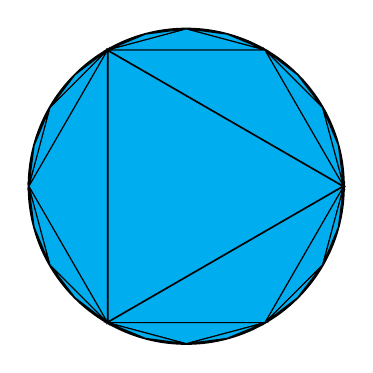
\begin{tikzpicture}[style=thick]
      \draw[fill=green] (0,0) circle (2);
      \pause
     % \draw             (1.0, -0.2) node{a};
      \path[draw,fill=cyan] (0:2)
      \foreach \x in {120,240}
        { -- (\x:2) } -- cycle;
      
      %\foreach \y in {0, 120, 240}
      %{
      %  \path[draw,fill=cyan] (\y:2)
      %  \foreach \x in {0,60,120}
      %   { -- (\x+\y:2) } -- cycle;
      %}
      \foreach \k in {3,6,12}
      { 
        \pause
        \foreach \x [evaluate=\x as \xx using (\x-1)*360/\k] in {1, ..., \k}
        { \path[draw,fill=cyan,style=thin] (\xx:2) 
          %\node{\x} at (\xx:2);
          \foreach \y [evaluate=\y as \yy using \xx+\y*360/\k/2] in {0,1,2}
          { -- (\yy:2) }
          -- cycle;
        }
      }
     \end{tikzpicture}
  \end{center}
  \end{minipage}%
  \begin{minipage}{0.45\linewidth}
    $\only<2-5>{A \leq A_1}
       \only<3-5>{+ 3A_2}
       \only<4-5>{+ 6 A_3}
       \only<5-5>{+ 12 A_4}$
    $\only<6>{A = A_1 + 3\sum_{n=0}^\infty 2^n A_{n+2}}$
  \end{minipage}
\end{frame}

%\setbeamercovered{transparent}
\begin{frame}{Why Measure Theory?}
  \note[item]{Now let's sum up, what we have gained from our intuitive
    thinking on volume}
    \begin{definition}
      A volume is a function $\mathcal{P}(\RR^n) \to [0, \infty]$ such that
      \begin{enumerate}[<+-| alert@+>]
      \item Positivity: $\mu_n(A) \geq 0$ for all $A \subset \RR^n$.
        \note[item]{First, we want it to be positive (remember, we are talking
          about subsets. There is no way to distinguis $[a,b]$ from $[b,a]$
          right now}
      \item Congruence: $\mu_n(A) = \mu_n(B)$ for all congruent $A$ and $B$.
        \note[item]{Furthermore, we want it to be invariant under congruences.
          That is, it should not change under rotation and mirroring. Otherwise
          the example with the triangle would not work}
      \item Norm: $\mu_n([0,1]^n) = 1$.
        \note[item]{Then, we want one volume fixed: The one of the unit
          square.}
      \item $\sigma$-Additivity: $\mu_n(\bigcup_{i=1}^{\infty} A_i) =
        \sum_{i=1}^\infty \mu_n(A_i)$ for disjoint $A_i$.
        \note[item]{And finally, we want it to be additive. But not only
          for finite unions, but even for countable unions. We need this
          property to be able to calculate the volume of the circle in
          the way I outlined.}
      \end{enumerate}
    \end{definition}
    %\pause
    \begin{lemma}<+->
      \begin{enumerate}
      \item $\mu_n(\{x\}) = 0$
      \item $\mu_n(A) \leq \mu_n(B)$ for $A \subseteq B$.
      \end{enumerate}
    \end{lemma}
    \note[item]{From this properties, we already gain to important statements,
      that we don't have to demand in addition: Points have volume 0 and
      the volume is monoton: If one shape contains another one, it has
      to have at least the same volume.}

\end{frame}

\begin{frame}{The vitali set}
  \note[item]{Okay, now that we know how we would like our volume function
    to behave, we just have to find it. More precisely, mathematicians
    want to show that it exists and that it is unique. Till know,
    basically, there could be more than one volume functions with this
    property.}
  \note[item]{This is what the mathematicians were
  Let $V$ be a set of representatives for the quotient group $\RR/\QQ$
  from $[0,1]$, that is: For every $z \in \RR$, there is exactly one
  element of $z+\QQ$ in $V$ and this element lies within $[0,1]$.

  \begin{lemma}
    \begin{enumerate}
    \item For $p\neq q$, $p,q\in\QQ$  we
      have $p+V \cap q+V = \emptyset$.
    \item Let $(p_n)_{n\in\NN}$ an enumeration of the rational numbers
      in $[-1,1]$ and $V_n=p_n + V$, then we have $[0,1] \subset
      \bigcup_{n=1}^{\infty} V_n \subset [-1, 2]$.
    \end{enumerate}
  \end{lemma}
\end{frame}

\begin{frame}{The Vitali set}

  Since $[0,1] \subset \bigcup_{n=1}^{\infty} V_n \subset [-1, 2]$, we have by
  monotony of the volume
  
  \[1 \leq \sum_{n=1}^\infty \mu_1(V_n) \leq 3,\]
  \pause
  but by congruence we have $\mu_1(V_n) = \mu_1(V)$ for all $n$, therefore

  \[1 \leq \sum_{n=1}^\infty \mu_1(V) \leq 3.\]

  \pause
  But if $\mu_1(V)=0$ then $\sum_{n=1}^\infty \mu_1(V)=0$ and if
  $\mu_1(V)>0$ then $\sum_{n=1}^\infty \mu_1(V) = \infty$. Therefore
  such a $\mu_1$ cannot exist.

\end{frame}

\begin{frame}{The Banach-Tarski Paradox}
  \begin{theorem}[Banach-Tarski]
    Given a solid sphere in 3-dimensional space, there exists a decomposition of
    the sphere into five disjoint subsets (i.\,e., non-overlapping pieces),
    which can be put back together in a different way (only using isometries) to
    yield two identical copies of the original sphere.
  \end{theorem}
  \pause
  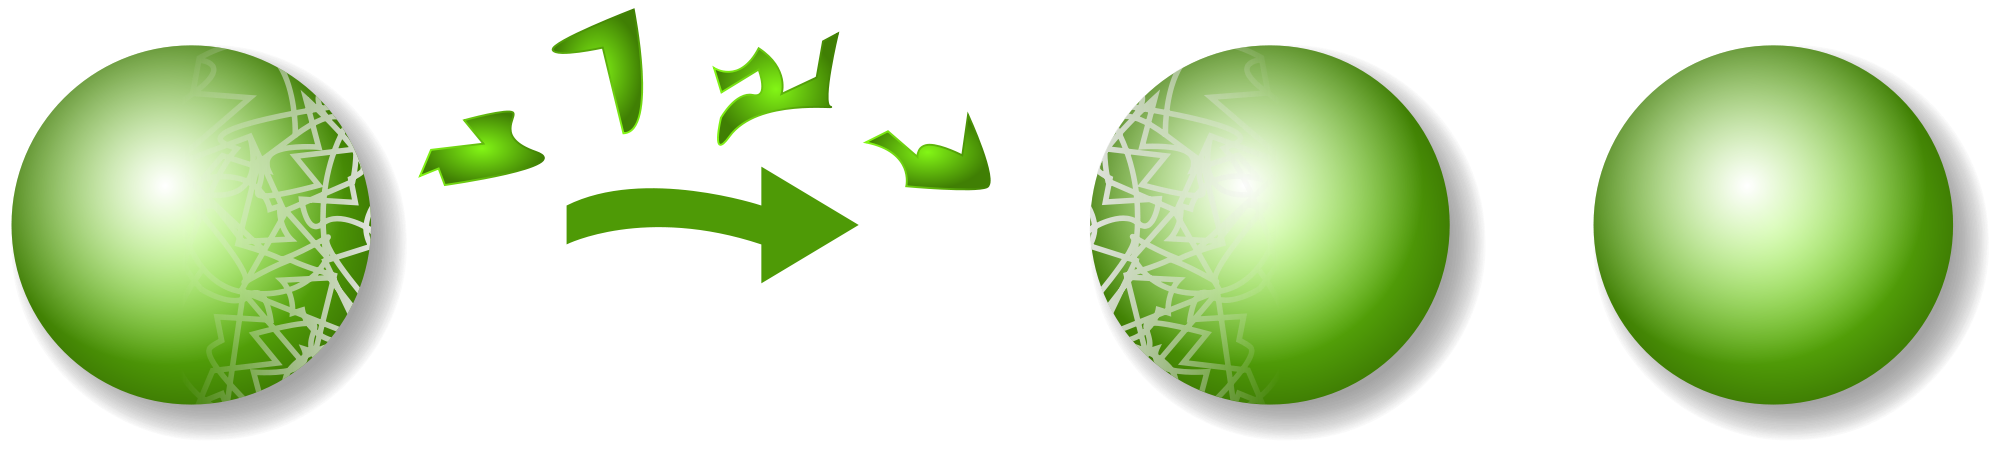
\includegraphics[width=\linewidth]{Banach-Tarski_Paradox-Illustration.png}
  \rotatebox{90}{\tiny{Source: Wikipedia}}
\end{frame}

\begin{frame}{The Banach-Tarski Paradox}
  \begin{itemize}
  \item Proof is a little bit technical, but perfectly understandable
     with very little mathematical background
  \item Ingrediences
    \begin{itemize}
    \item Shifting to infinity (``Trick of Hilbert's Hotel'')
    \item Paradoxial decomposition of a group generated by two rotations $f$ and $g$ into $I$, $J$, $K$, i.\,e., such that $fI = J \cup K$, $gI = J$, $g^2I = K$
    \item Axiom of choice
    \end{itemize}
  \end{itemize}
\end{frame}

\section{Measure Theory}

\begin{frame}{So far}
  \begin{itemize}
  \item We cannot have volume function for all subsets of $\RR^n$.
  \item Solution: Define it only on a specific set of subsets.
  \item This subset has to have certain properties to enable us
    to do the usual calculations for volumes
  \end{itemize}
\end{frame}

\begin{frame}{$\sigma$-algebras}
  \begin{definition}[$\sigma$-algebra]
    Let $\Omega$ be a set. Then a set $\mathcal{A} \subset \mathcal{P}(\Omega)$
    is called $\sigma$-algebra, if it satisfies the following properties:
    \begin{enumerate}
    \item $\Omega \in \mathcal{A}$
    \item Closed under complements: $X \in \mathcal{A} \Rightarrow
      \Omega\setminus X \in \mathcal{A}$
    \item Closed under countable unions: If $X_n \in \mathcal{A}$ for all $n$,
      then $\bigcup_{n=1}^\infty X_n \in \mathcal{A}$.
    \end{enumerate}
  \end{definition}

  \begin{example}
    \begin{enumerate}
    \item Borel $\sigma$-algebra $\mathcal{B}$ generated by all intervals
      $[a,b]$ on $\RR$.
    \end{enumerate}
  \end{example}
\end{frame}

\begin{frame}{Measures}
  \begin{definition}[measure]
    Let $\Omega$ be a set and $\mathcal{A}$ be a $\sigma$-algebra on
    $\Omega$. Then a function $\mu: \mathcal{A} \to [0, \infty]$ is called a
    measure, if:
    \begin{enumerate}
    \item $\mu(\emptyset) = 0$
    \item $\sigma$-additivity: If $X_n \in \mathcal{A}$ are pairwise disjoint,
      then $\mu(\bigcup_n X_n) = \sum_n \mu(X_n)$.
    \end{enumerate}
  \end{definition}

  \begin{example}
    \begin{enumerate}
    \item Lebesgue measure $\mu$ on $\RR$ with $\mathcal{B}$: The extension of
      $\mu([a,b])=b-a$ to $\mathcal{B}$ (it is all but trivial that it exists
      and is well-defined).
    \item Counting measure on $\NN$ with $\mathcal{P}(\NN)$
    \item Delta-measure $\delta$ on $\RR$: $\delta(X)=1$ if and only if $0 \in
      X$, else 0.
    \end{enumerate}
  \end{example}
\end{frame}

\begin{frame}{Integration theory}
  \begin{definition}[measurable function]
    Let $\Omega_1$, $\Omega_2$ be sets with $\sigma$-algebras $\mathcal{A}_1$,
    $\mathcal{A}_2$. Then a function $f: \Omega_1 \to \Omega_2$ is called
    \textit{measurable}, if $f^{-1}(X) \in \mathcal{A}_1$ for all $X \in
    \mathcal{A}_2$.
  \end{definition}
  \begin{itemize}
  \item Important for integration: The measure integral divides
     horizontal, not vertical
  \end{itemize}
\end{frame}

\begin{frame}{Integration theory}
  Let $f: \Omega \to \RR$ be measurable and elementary: It takes only finitely many values $\alpha_i$ on the disjoint measurable sets $A_i$. Then we define
  \[
    \int_{\Omega} f\td \mu := \sum_{i=1}^n \alpha_i\mu(A_i)
  \]

  \begin{center}
    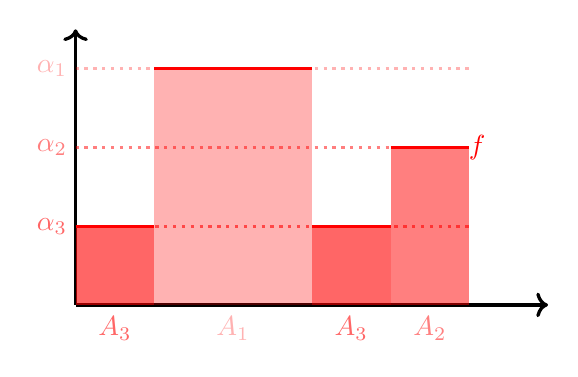
\begin{tikzpicture}[style=very thick]
      \draw[->] (0,0) -- (6,0);
      \draw[->] (0,0) -- (0,3.5);
      \draw[red] (0,1) -- (1,1)
                 (1,3) -- (3,3)
                 (3,1) -- (4,1)
                 (4,2) -- (5,2);
      \draw[red] (5.1,2) node{$f$};
      %\pause
      \visible<2->{
      \fill[fill=red,opacity=0.3] (1,0) rectangle (3,3);
      \draw[red,opacity=0.3] (2,-0.3) node{$A_1$};
      \draw[red,opacity=0.3] (-0.3,3) node{$\alpha_1$};
      \draw[dotted,red,opacity=0.3] (0,3) -- (5,3);}
      %\pause

      \visible<3->{
      \fill[fill=red,opacity=0.5] (4,0) rectangle (5,2);
      \draw[red,opacity=0.5] (4.5,-0.3) node{$A_2$};
      \draw[red,opacity=0.5] (-0.3,2) node{$\alpha_2$};
      \draw[dotted,red,opacity=0.5] (0,2) -- (5,2);}
      %\pause
      \visible<4->{
      \fill[fill=red,opacity=0.6] (0,0) rectangle (1,1);
      \fill[fill=red,opacity=0.6] (3,0) rectangle (4,1);
      \draw[red,opacity=0.6] (0.5,-0.3) node{$A_3$};
      \draw[red,opacity=0.6] (3.5,-0.3) node{$A_3$};
      \draw[red,opacity=0.6] (-0.3,1) node{$\alpha_3$};
      \draw[dotted,red,opacity=0.6] (0,1) -- (5,1);}
    \end{tikzpicture}
  \end{center}
\end{frame}

\begin{frame}{Integration theory}
  By a limit process (formal completion), the integral is extended to a space
  $L_1$ of integrable ``functions''.
  \begin{center}
    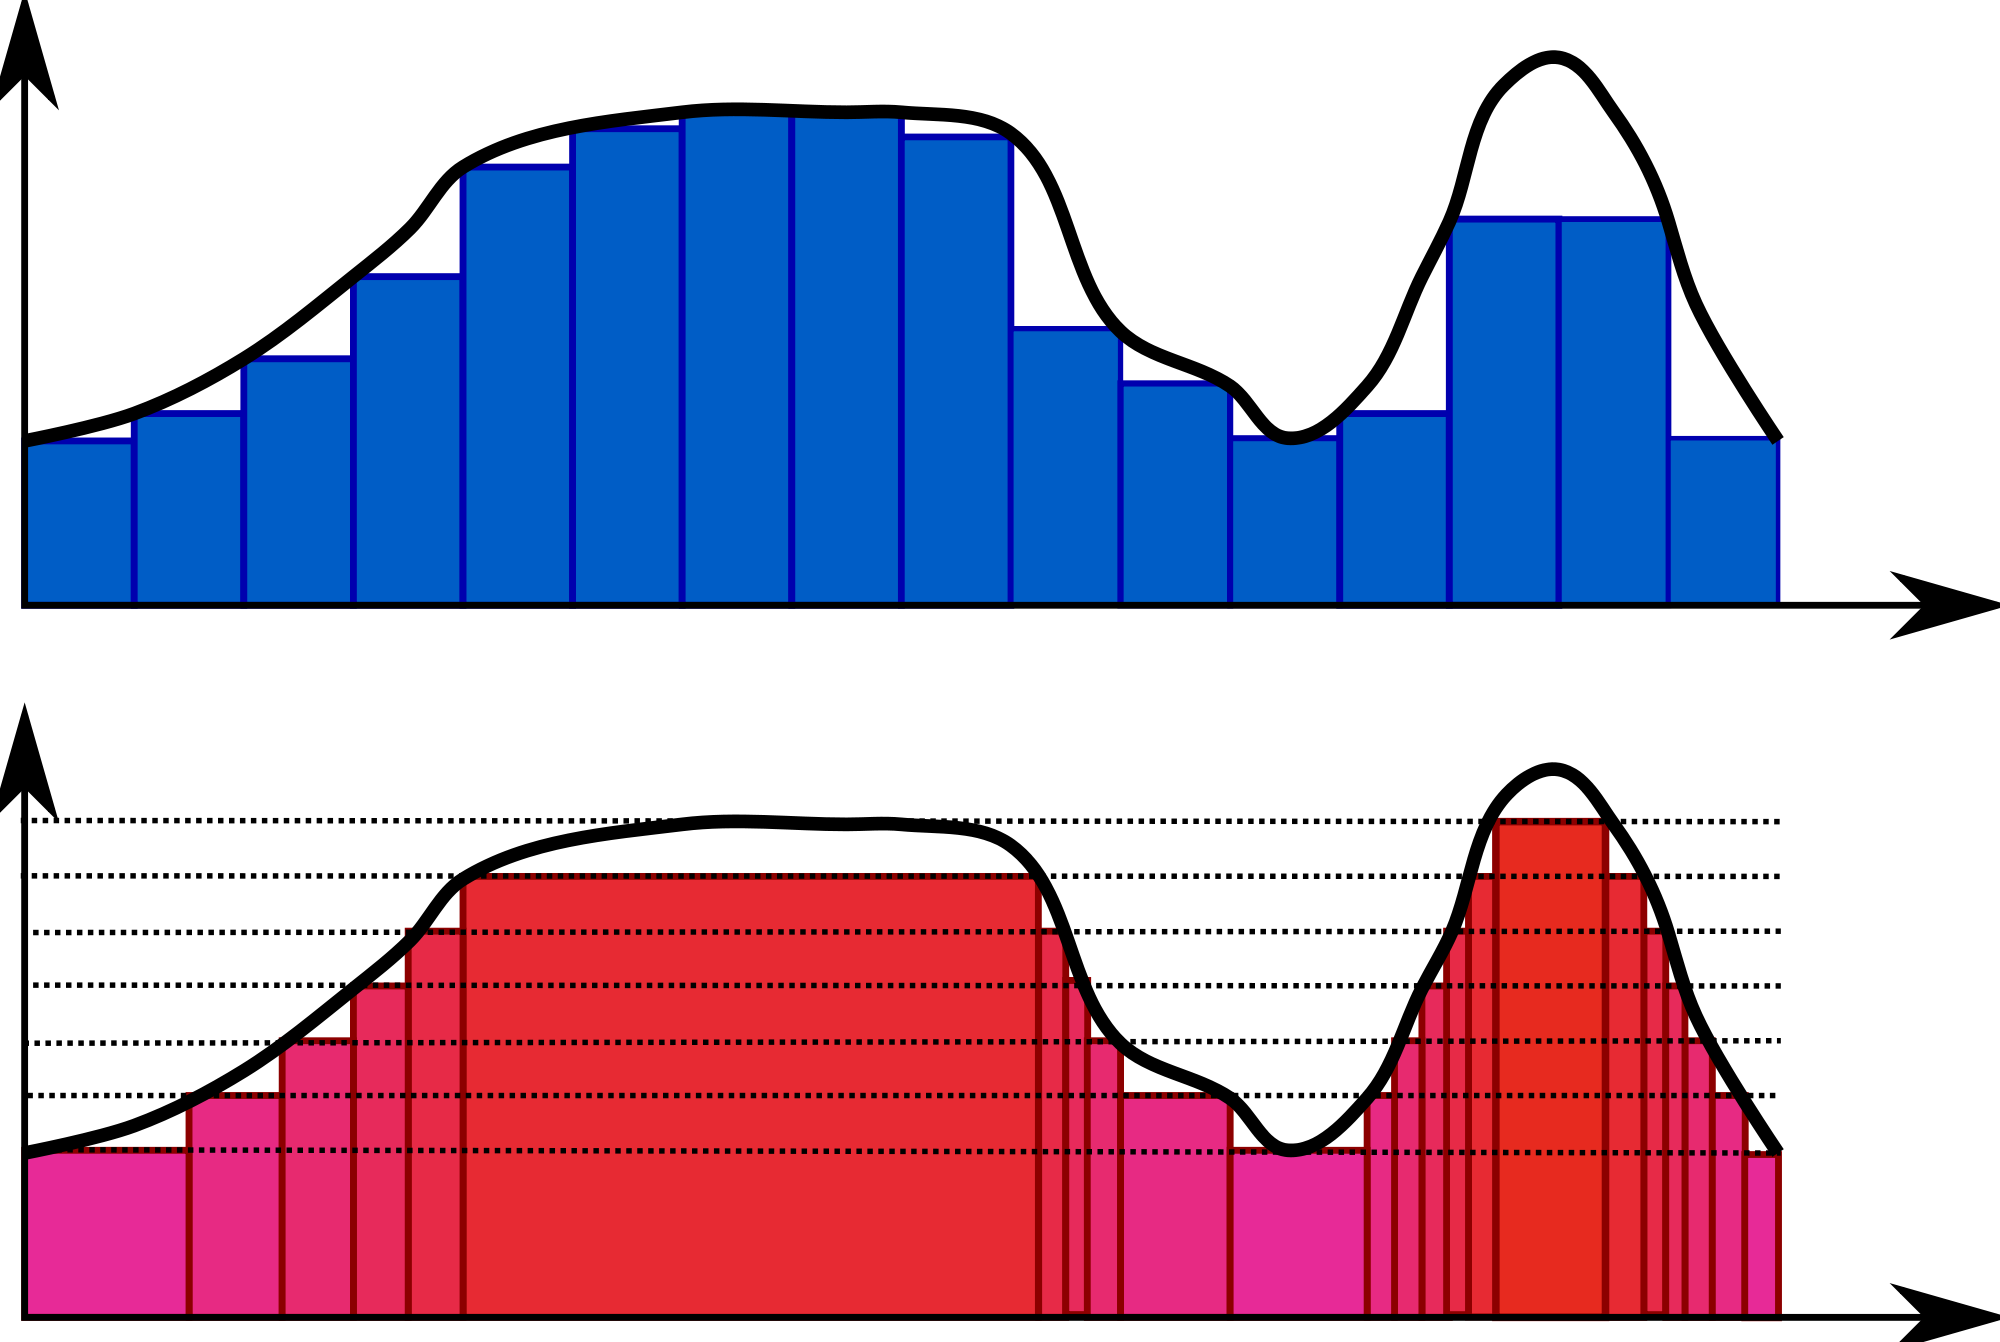
\includegraphics[width=0.7\linewidth]{Riemannvslebesgue.png}
    \rotatebox{90}{\tiny Wikipedia}
  \end{center}
\end{frame}

\begin{frame}{Integration theory}
  \begin{itemize}
  \item More integrable functions: $\int_\RR \chi_\QQ \td x= 0$.
  \item Much better convergence properties, e.\,g. dominated convergence: $f_n
    \in L_1$, $f_n \to f$ pointwise and $|f_n|\leq g$ for some $g \in L_1$, then
    $f \in L_1$ and $\int f = \lim \int f_n$ (For comparison: The Riemann
    integral needs uniform convergence for this property).
  \end{itemize}
\end{frame}

\section{Probability Theory}

\begin{frame}{Probability theory}
  
\end{frame}

\end{document}
